
\Literature: \cite{mumc03,chpe15,momu06,muso11}

\subsubsection{Tensor invariants}\label{sec:invariants}

Before we dive into the world of nonlinear rheologies it is necessary to introduce the concept of tensor 
invariants since they are needed further on. \index{general}{tensor invariant}
Unfortunately there are many different notations used in the literature and these can prove to be 
confusing. Note that we only consider symmetric tensors in what follows.

\index{general}{Moment Invariant}
Given a tensor $\bm{T}$,  one can compute its (moment) invariants as follows \cite[p.339]{reddybook2}: 
\begin{itemize}
\item first invariant:
\begin{eqnarray}
{\cal I}_1({\bm T})|^{2D} &=& Tr[\bm{T}] = T_{xx} + T_{yy} \nonumber\\
{\cal I}_1({\bm T})|^{3D} &=& Tr[\bm{T}] = T_{xx} + T_{yy} + T_{zz} 
\end{eqnarray}
\item second invariant:
\begin{eqnarray}
{\cal I}_2({\bm T})|^{2D} &=& \frac{1}{2} Tr[{\bm{T}^2}] = \frac{1}{2} \sum_{ij} T_{ij} T_{ji} = \frac{1}{2} (T_{xx}^2 + T_{yy}^2) + T_{xy}^2 \nonumber\\
{\cal I}_2({\bm T})|^{3D} &=& \frac{1}{2} Tr[{\bm{T}^2}] = \frac{1}{2} \sum_{ij} T_{ij} T_{ji} = \frac{1}{2} (T_{xx}^2 + T_{yy}^2 + T_{yy}^2) + T_{xy}^2 + T_{xz}^2 + T_{yz}^2 
\end{eqnarray}
\item third invariant: 
\begin{equation}
{\cal I}_3({\bm T}) = \frac{1}{3} Tr[{\bm{T}^3}]  = \frac{1}{3}\sum_i\sum_j \sum_k T_{ij} T_{jk} T_{ki} 
\end{equation}
\end{itemize}


The implementation of the plasticity criterions relies essentially 
on the second invariants of the (deviatoric) stress ${\bm \tau}$ and the (deviatoric) strainrate tensors $\dot{\bm \varepsilon}$:

\begin{eqnarray}
{\cal I}_2({\bm \tau})|^{2D}            
&=& \frac{1}{2} ( \tau_{xx}^2 + \tau_{yy}^2  ) + \tau_{xy}^2   \nonumber\\
&=& \frac{1}{4} (\sigma_{xx} - \sigma_{yy})^2 + \sigma_{xy}^2 \nonumber\\
&=& \frac{1}{4} (\sigma_{1} - \sigma_{2})^2 \nonumber\\
\nonumber\\
{\cal I}_2({\bm \tau})|^{3D}            
&=&\frac{1}{2}(\tau_{xx}^2 + \tau_{yy}^2 + \tau_{zz}^2 ) + \tau_{xy}^2 + \tau_{xz}^2 + \tau_{yz}^2  \nonumber\\
&=&\frac{1}{6}\left[(\sigma_{xx}-\sigma_{yy})^2 + (\sigma_{yy}-\sigma_{zz})^2 + (\sigma_{xx}-\sigma_{zz})^2 \right] 
   + \sigma_{xy}^2 + \sigma_{xz}^2 + \sigma_{yz}^2 \nonumber \\
&=&\frac{1}{6}\left[(\sigma_{1}-\sigma_{2})^2 +(\sigma_{2}-\sigma_{3})^2 + (\sigma_{1}-\sigma_{3})^2 \right] \nonumber\\
\nonumber\\
{\cal I}_2(\dot{\bm{\varepsilon}}^d)|^{2D} 
&=& \frac{1}{2} \left[ (\dot{\varepsilon}_{xx}^d)^2 + (\dot{\varepsilon}_{yy}^d)^2  \right] + (\dot{\varepsilon}_{xy}^d)^2  \nonumber\\
           &=& \frac{1}{2} \left[ 
               \frac{1}{4}(\dot{\varepsilon}_{xx} - \dot{\varepsilon}_{yy})^2 + \frac{1}{4}(\dot{\varepsilon}_{yy} - \dot{\varepsilon}_{xx})^2 
               \right] + \dot{\varepsilon}_{xy}^2  \nonumber\\
           &=& \frac{1}{4} (\dot{\varepsilon}_{xx} - \dot{\varepsilon}_{yy})^2  + \dot{\varepsilon}_{xy}^2  \nonumber\\
\nonumber\\
{\cal I}_2(\dot{\bm{\varepsilon}}^d)|^{3D} 
&=& \frac{1}{2} \left[ (\dot{\varepsilon}_{xx}^d)^2 + (\dot{\varepsilon}_{yy}^d)^2 + (\dot{\varepsilon}_{zz}^d)^2   \right] 
+ (\dot{\varepsilon}_{xy}^d)^2  
+ (\dot{\varepsilon}_{xz}^d)^2  
+ (\dot{\varepsilon}_{yz}^d)^2  \nonumber\\
           &=& \frac{1}{6} \left[ (\dot{\epsilon}_{xx}-\dot{\epsilon}_{yy})^2 + (\dot{\epsilon}_{yy}-\dot{\epsilon}_{zz})^2 + (\dot{\epsilon}_{xx}-\dot{\epsilon}_{zz})^2 \right] 
               + \dot{\epsilon}_{xy}^2 + \dot{\epsilon}_{xz}^2 + \dot{\epsilon}_{yz}^2 \nonumber \\
\nonumber
\end{eqnarray}

Note that these (second) invariants are almost always used under a square root so we define:
\begin{mdframed}[backgroundcolor=blue!5]
\[
\tau_{e}=\sqrt{{\cal I}_2({\bm \tau})}
\quad\quad
\quad\quad
\dot{\varepsilon}_{e}=\sqrt{{\cal I}_2(\dot{\bm \varepsilon}^d)}
\]
\end{mdframed}
Note that these quantities have the same dimensions as their tensor counterparts, i.e. Pa for stresses and s$^{-1}$ for strain rates.



The third (deviatoric) stress invariant is given by: (VERIFY!!)
\begin{eqnarray}
{\cal I}_3({\bm \tau})|^{3D} 
&=&  \frac{1}{3} s_{xx} (s_{xx}^2 + 3  s_{xy}^2   + 3  s_{xz}^2  )     \nonumber\\
&+& \frac{1}{3} s_{yy} (3s_{xy}^2 +  s_{yy}^2   + 3  s_{yz}^2  )     \nonumber\\
&+& \frac{1}{3} s_{zz} ( 3 s_{xz}^2  + 3 s_{yz}^2 +s_{zz}^2)       \nonumber\\
&+& 2   s_{xy} s_{xz} s_{yz}   \nonumber \\
&=& s_1 s_2 s_3 \nonumber
\end{eqnarray}








%%%%%%%%%%%%%%%%%%%%%%%%%%%%%%%%%%%%%%%%%%%%%%%%%%%%%%%%%%%%%%%%%%%%%%%%%%%%%%%%%%%%%%%%%%%%%%%%%%%%%%%%%%%%%%%%%%%%%%%%%%%
\subsubsection{Scalar viscoplasticity}

This formulation is quite easy to implement. It is widely used, e.g. \cite{will92,thfb08,spmw16}, and relies on the assumption that 
a scalar quantity $\eta_p$ (the 'effective plastic viscosity') exists such that the deviatoric stress tensor 
\begin{equation}
{\bm \tau}=2\eta_p \dot{\bm\varepsilon} \label{eqscpl1}
\end{equation}
is bounded by some yield stress value $Y$.
From Eq. (\ref{eqscpl1}) it follows that $\underline{\tau}_{II}= 2\eta_p \dot{\underline{\varepsilon}}_{II}=Y$ which yields
\begin{mdframed}[backgroundcolor=blue!5]
\[
\eta_p = \frac{Y}{2 \dot{\underline{\varepsilon}}_{II}}
\]
\end{mdframed}
This approach has also been coined the Viscosity Rescaling Method (VRM) \cite{kacha04}. 
\index{general}{VRM} \index{general}{Viscosity Rescaling Method}

\improvement[inline]{insert here the rederivation 2.1.1 of spmw16}

It is at this stage important to realise that (i) in areas where the strainrate is low, the resulting effective viscosity will be large, and 
(ii) in areas where the strainrate is high, the resulting effective viscosity will be low. This is not without consequences since 
(effective) viscosity contrasts up to 8-10 orders of magnitude have been observed/obtained with this formulation and it makes the FE 
matrix very stiff, leading to (iterative) solver convergence issues.
In order to contain these viscosity contrasts one usually resorts to viscosity limiters $\eta_{min}$ and $\eta_{max}$ such that 
\[
\eta_{min} \leq \eta_p \leq \eta_{max}
\]
Caution must be taken when choosing both values as they may influence the final results.


\begin{mdframed}[backgroundcolor=green!5]
\begin{itemize}
\item[$\triangleright$] {\sl python\_codes/fieldstone\_indentor}
\end{itemize}
\end{mdframed}


%-------------------------------------------------
\subsubsection{About the yield stress value $Y$}

In geodynamics the yield stress value is often given as a simple function. 
It can be constant (in space and time) and in this case we are dealing with a von Mises plasticity yield criterion. 
\index{general}{von Mises}. We simply assume $Y_{vM}=C$ where $C$ is a constant cohesion independent of pressure, strainrate,
deformation history, etc ... \index{general}{cohesion}

Another model is often used: the Drucker-Prager plasticity model. \index{general}{Drucker-Prager}
A friction angle $\phi$ is then introduced and the yield value $Y$ takes the form
\[
Y_{DP}=p \sin\phi + C \cos \phi
\]
and therefore depends on the pressure $p$. Because $\phi$ is with the range $[0^\circ,45^\circ]$, $Y$ is
found to increase with depth (since the lithostatic pressure often dominates the overpressure).

Note that a slightly modified verion of this plasticity model has been used: the total pressure $p$
is then replaced by the lithostatic pressure $p_{lith}$.




%-------------------------------------------------
\subsubsection{Work in progress}

\Literature \cite{zico74,zigo74,zico74b,zien75,corm75,zigo75,zihl75,zijo78,vidm82,vidm84,vede84,zivt85,vimd86}
\cite{wasd97,debo88,debo01,hesd02,bewv11,mumg10}


\begin{center}
\begin{minipage}[t]{0.5\textwidth}

\begin{center}
\begin{tikzpicture}
%\draw[fill=gray!23,gray!23](0,0) rectangle (7,4);
%\draw[step=0.5cm,gray,very thin] (0,0) grid (7,4); %background grid

\draw[thick] (0.5,2.5) -- (2,2.5) ;  
\draw[thick] (2.5,2.5) -- (4,2.5) ;  
\draw[thick] (4.5,2.5) -- (5.5,2.5) ;  

\draw[thick] (1.5,3) -- (2.5,3) -- (2.5,2) -- (1.5,2);  
\draw[thick] (3.5,3) -- (4.5,3) -- (4.5,2) -- (3.5,2);  

\node[] at (2,1.5) {$\eta_1$};
\node[] at (4,1.5) {$\eta_2$};

%--------------------------------------------------------

\draw[thick] (6.5,2.5) -- (7.5,2.5) ;  
\draw[thick] (10.5,2.5) -- (11.5,2.5) ;  

\draw[thick] (9,3.5) -- (7.5,3.5) -- (7.5,1.5) -- (9,1.5);  
\draw[thick] (9.5,3.5) -- (10.5,3.5) -- (10.5,1.5) -- (9.5,1.5);  


\draw[thick] (8.5,4) -- (9.5,4) -- (9.5,3) -- (8.5,3);  
\draw[thick] (8.5,2) -- (9.5,2) -- (9.5,1) -- (8.5,1);  

\node[] at (9.8,4) {$\eta_1$};
\node[] at (9.8,1) {$\eta_2$};

%\draw[thick] (1,1) -- (3,1.2) -- (2.7,3) -- (1.1,3.1) -- cycle;  
%\node[] at (0.8,0.8) {0};
%\node[] at (3.2,1) {1};
%\node[] at (2.9,3.1) {2};
%\node[] at (0.9,3.2) {3};
%\draw[black,fill=black] (1,1)     circle (2pt); \draw (1,1) circle (4pt);
%\draw[black,fill=black] (3,1.2)   circle (2pt); \draw (3,1.2) circle (4pt);
%\draw[black,fill=black] (2.7,3)   circle (2pt); \draw (2.7,3) circle (4pt);
%\draw[black,fill=black] (1.1,3.1) circle (2pt); \draw (1.1,3.1) circle (4pt);
%\draw[black,fill=black] (3.1,0.2) circle (2pt); \node[] at (3.4,0.2) {$\vec\upnu$};
%\draw (4.1,0.2) circle (4pt); 
%\node[] at (2.5,4.5) {4 vel. nodes, 4 press. nodes};
\end{tikzpicture}\\
\end{center}

\end{minipage}
\end{center}
\begin{itemize}
\item Two dashpots/dampers in series: 
\[
\dot{\varepsilon}_1 = \sigma/{2 \eta_1} 
\qquad
\dot{\varepsilon}_2 = \sigma/{2 \eta_2} 
\qquad
\dot{\varepsilon} = \sigma/{2 \eta_{eff}} 
\]
\[
\dot{\varepsilon} = \dot{\varepsilon}_1 + \dot{\varepsilon}_2
\Rightarrow
\sigma/{2 \eta_{eff}} = \sigma/{2 \eta_1} + \sigma/{2 \eta_2} 
\]
so
\[
\eta_{eff} = \left( \frac{1}{\eta_1} + \frac{1}{\eta_2} \right)^{-1}
\]
\item Two dashpots/dampers in parallel: 
\[
\eta_{eff} = \eta_1 + \eta_2
\]
\end{itemize}

One could consider the following arrangement of dashpots and plastic elements:

\begin{center}
\begin{minipage}[t]{0.5\textwidth}

\begin{center}
\begin{tikzpicture}
%\draw[fill=gray!23,gray!23](0,0) rectangle (7,5);
%\draw[step=0.5cm,gray,very thin] (0,0) grid (7,5); %background grid

\draw[thick] (0.5,2.5) -- (2,2.5) ;  
\draw[thick] (2.5,2.5) -- (4.5,2.5) ;  
\draw[thick] (7.5,2.5) -- (9,2.5) ;  

\draw[thick] (1.5,3) -- (2.5,3) -- (2.5,2) -- (1.5,2);  
\draw[thick] (5.5,4) -- (6.5,4) -- (6.5,3) -- (5.5,3);  

\node[] at (2,1.6) {$\eta_M$};
\node[] at (6,4.4) {$\eta_m$};

\draw[thick] (6,3.5) -- (4.5,3.5) -- (4.5,1.5) -- (5,1.5);  
\draw[thick] (6.5,3.5) -- (7.5,3.5) -- (7.5,1.5) -- (7,1.5);  

\draw[thick] (5,1.5) -- (5.5,1.4) -- (6.5,1.4) ;  
\draw[thick] (5.5,1.6) -- (6.5,1.6) -- (7,1.5) ;  

\node[] at (6,1.) {$c$};


%\draw[thick] (1,1) -- (3,1.2) -- (2.7,3) -- (1.1,3.1) -- cycle;  
%\node[] at (0.8,0.8) {0};
%\node[] at (3.2,1) {1};
%\node[] at (2.9,3.1) {2};
%\node[] at (0.9,3.2) {3};
%\draw[black,fill=black] (1,1)     circle (2pt); \draw (1,1) circle (4pt);
%\draw[black,fill=black] (3,1.2)   circle (2pt); \draw (3,1.2) circle (4pt);
%\draw[black,fill=black] (2.7,3)   circle (2pt); \draw (2.7,3) circle (4pt);
%\draw[black,fill=black] (1.1,3.1) circle (2pt); \draw (1.1,3.1) circle (4pt);
%\draw[black,fill=black] (3.1,0.2) circle (2pt); \node[] at (3.4,0.2) {$\vec\upnu$};
%\draw (4.1,0.2) circle (4pt); 
%\node[] at (2.5,4.5) {4 vel. nodes, 4 press. nodes};
\end{tikzpicture}\\
\end{center}

\end{minipage}
\end{center}

 which yields the following effective viscosity:
\[
\eta_{eff} = \left( \frac{1}{\eta_M}  + \frac{1}{\frac{c}{2 \dot{\varepsilon}_e} + \eta_m}  \right)^{-1}
\]
When the strain rate becomes very small,  $\dot{\varepsilon}_e \rightarrow 0$, $\eta_{eff}\rightarrow \eta_{M}$.
When the strain rate becomes very large,  $\dot{\varepsilon}_e \rightarrow \infty$, $\eta_{eff}\rightarrow \eta_{m}$.
We can then rewrite the above equation as a function of $\eta_{min}$ and $\eta_{max}$:
\[
\eta_{eff} = \left( \frac{1}{\eta_{max}}  + \frac{1}{\frac{c}{2 \dot{\varepsilon}_e} + \eta_{min}}  \right)^{-1}
\]

The effective viscosity is plotted here for various values of the minimum viscosity (for $c$=200MPa and $\eta_{max}=10^{25}Pa.s$:

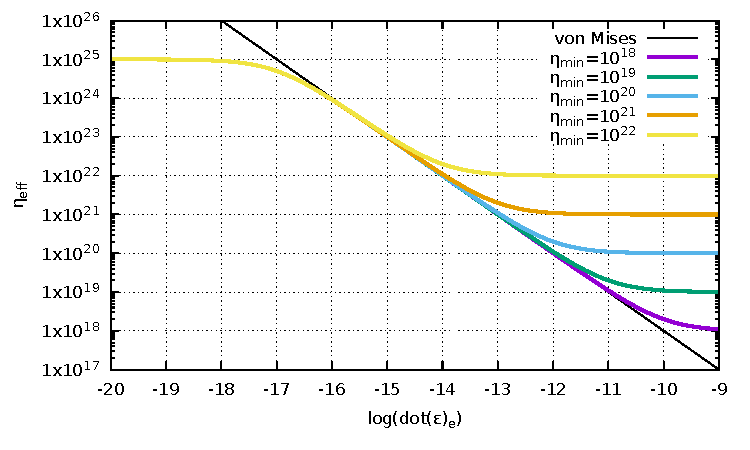
\includegraphics[width=8cm]{images/viscoplasticity/nu_eff}




Note that \cite{vidm82,vidm84,vimd86,zivt85} use the following formulation which they attribute to \cite{zijo78}:
\[
\eta_{eff} = \frac{c + (\dot{\varepsilon}_e / \gamma)^{1/n}}{ \dot{\varepsilon}_e }
\] 
For a perfectly plastic flow law, $\gamma \rightarrow \infty$ and then 
\[
\eta_{eff} = \frac{c}{ \dot{\varepsilon}_e }
\] 
and when when $c=0$ then the effective viscosity is essentially of the power law type.
Also, when $n=1$ the formulation becomes identical to the v-vp formulation (when the max viscosity is infinite) and with $1/\gamma=\eta_{min}$.





